%
% lorenz-definition.tex -- Definitionsgebiet des Lorenz-Modells
%
% (c) 2018 Prof Dr Andreas Müller, Hochschule Rapperswil
%
\documentclass[tikz]{standalone}
\usepackage{times}
\usepackage{txfonts}
\usepackage[utf8]{inputenc}
\usepackage{graphics}
\usetikzlibrary{arrows,intersections}
\begin{document}
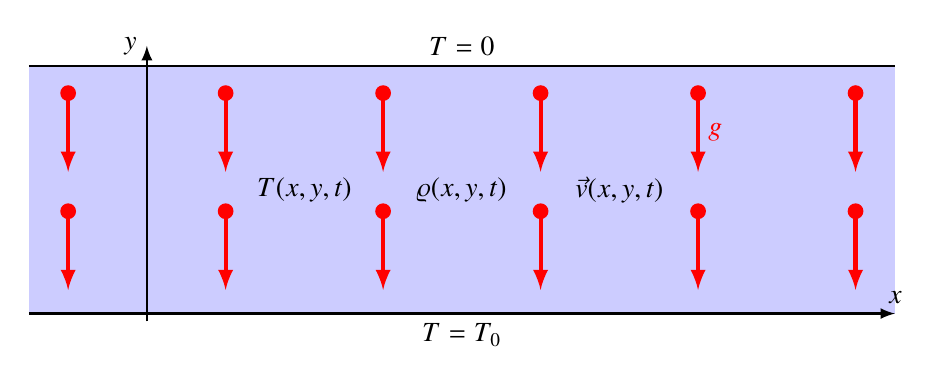
\begin{tikzpicture}[thick, >= latex]

\fill[color=blue!20] (-5.5,0)--(5.5,0)--(5.5,3.14)--(-5.5,3.14)--cycle;

\draw[->] (-5.5,0)--(5.5,0) coordinate[label=$x$];
\draw (-5.5,3.14)--(5.5,3.14);

\draw[->] (-4,-0.1)--(-4,3.4) coordinate[label={left:$y$}];

\node at (0,3.14) [above] {$T=0$};
\node at (0,0) [below] {$T=T_0$};

\node at (-2,1.57) {$T(x,y,t)$};
\node at (0,1.57) {$\varrho(x,y,t)$};
\node at (2,1.57) {$\vec{v}(x,y,t)$};

\foreach \y in {2.8,1.3}{
	\foreach \x in {-5,-3,...,5}{
		\fill[color=red] ({\x},{\y}) circle[radius=0.1];
		\draw[->,color=red,line width=1.5pt] ({\x},{\y})--({\x},{\y-1});
	}
}
\node at (3,2.3) [right] {\color{red} $g$};

\end{tikzpicture}
\end{document}

